%Ich bin ein TeX Dokument
\documentclass{scrartcl} % KOMA-Script Dokumentenklasse Article
%Für Positionierung von Gleitumgebungen
\usepackage{scrhack}
% Warnung, falls noch einmal kompiliert werden muss
\usepackage[aux]{rerunfilecheck}
% Paket für Schriftarteinstellung, muss immer geladen werden
\usepackage{fontspec}
% Deutsche Spracheinstellungen, wichtig z. B. für korrekte Trennung
\usepackage[ngerman]{babel}
% mehr Pakete hier
\usepackage{amsmath}
\usepackage{amssymb}
\usepackage{mathtools}
%ISO Normen benutzen
\usepackage[
math-style=ISO,
bold-style=ISO,
sans-style=italic,
nabla=upright,
partial=upright,
]{unicode-math}
%Für korrekte Zahlen mit Einheiten
\usepackage[
locale=DE,
separate-uncertainty=true,
per-mode=symbol-or-fraction,
]{siunitx}
% Unterstützung für Links und PDF Metadaten
\usepackage[unicode]{hyperref}
\usepackage{bookmark}
%Für das Einbinden von Grafiken
\usepackage{graphicx}
%Positionierung von Gleitumgebungen
\usepackage{float}
%Für Tabellen
\usepackage{booktabs}
% Einstellungen hier, z.B. Fonts
\setmathfont{Latin Modern Math}
\floatplacement{figure}{H}
\floatplacement{table}{H}
%Für die Tabellen
\usepackage{booktabs}

\begin{document}
\title{Versuch D206 "Die Wärmepumpe"}
\author{Henry Krämerkämper \and Christopher Breitfeld}
\date{29.10.2020}
\maketitle
\newpage
\tableofcontents
\newpage
\section{Einleitung}
Der Versuch "Die Wärmepumpe", welcher im folgenden erklärt und durchgeführt wird, behandelt den Transport von
Wärmeenergie von einem kälteren zu einem wärmeren Reservoir. Nach dem zweiten Hauptsatz der Thermodynamik sind beide
Flussrichtungen möglich, nur ist für den Transport vom kälteren zum wärmeren Reservoir zusätzliche Arbeit nötig. Diese verrichtet die Wärmepumpe.
Im folgenden werden Merkmale dieser behandelt, in etwa die Güteziffer der Pumpe sowie ihr Massendurchsatz und der Wirkungsgrad des Kompressors.
\section{Theoretische Grundlagen}
Im folgenden wird immer der Differentialquotient anstelle des Differenzenquotienten verwendet, da alle Berechnungen auf einer nicht-linearen Ausgleichsrechnung fußen.
  \subsection{Die Güteziffer}
  \label{sec:güteziffer}
  Die hier verwendete Wärmepumpe wird unter anderem charakterisiert durch die Güteziffer $ v $. Sie gibt das Verhältnis zwischen der aufgewendeten Arbeit für den Wärmetransport
  $ A $ und der transportierten Wärmeenergie $ Q_\text{transp} $ an. Eine Formel für die Berechnung der Güteziffer lässt sich wie folgt herleiten: \\
  \\
  Wir bezeichnen die den wärmeren Reservoir 1 zugeführte Wärmeenergie als $ Q_\text{1} $ sowie die dem kälteren Reservoir 2 entnommene Wärmeenergie als $ Q_\text{2} $.
  Dann gilt nach dem ersten Hauptsatz der Thermodynamik
  \begin{equation}
    Q_\text{1} = Q_\text{2} + A.
    \label{eqn:wärmeenergie1}
  \end{equation}
  Dann ist das Verhältnis zwischen transportierter Wärmeenergie und aufgewendeter Arbeit
  \begin{equation}
    \frac{Q_\text{1}}{A} = v.
    \label{eqn:güteziffer}
  \end{equation}
  Um die Güteziffer einer idealen Wärmepumpe zu berechnen, betrachten wir die Zusammenhänge nach dem zweiten Hauptsatz der Thermodynamik:
  %Finde ich persönlich schwach formuliert, hier müsste nochmal nachgearbeitet werden
  \begin{equation}
    \frac{Q_\text{1}}{T_\text{1}} - \frac{Q_\text{2}}{T_\text{2}} = 0
    \label{eqn:wärmeenergie2}
  \end{equation}
  Gleichung \eqref{eqn:wärmeenergie2} gilt nur unter der Vorraussetzung, dass der Prozess reversibel abläuft.
  Da dies in der Realität nicht möglich ist, muss \eqref{eqn:wärmeenergie2} im Falle eines irreversiblen Prozesses
  anders formuliert werden:
  \begin{equation}
  	\frac{Q_\text{1}}{T_\text{1}} - \frac{Q_\text{2}}{T_\text{2}} > 0
  	\label{eqn:wärmeenergie3}
  \end{equation}
	Aus Gleichung \eqref{eqn:wärmeenergie1} und Gleichung \eqref{eqn:wärmeenergie3} sowie der Definition der Güteziffer
	\eqref{eqn:güteziffer} ergibt sich die Güteziffer einer idealen Wärmepumpe zu
	\begin{equation}
		v_\text{ideal} = \frac{Q_\text{1}}{A} = \frac{T_\text{1}}{T_\text{1} - T_\text{2}}
		\label{eqn:idealegüteziffer}
	\end{equation}
	Dann gilt analog zu \eqref{eqn:idealegüteziffer} für die reale Güteziffer:
	\begin{equation}
		v_\text{real} < \frac{T_\text{1}}{T_\text{1}-T_\text{2}}
		\label{eqn:realegüteziffer1}
	\end{equation}
  Die reale Güteziffer lässt sich auch aus dem Differentialquotienten $ \frac{\increment T_\text{1}}{\increment t}$ berechnen. Die transportierte Wärmemenge $\increment Q_\text{1}$
  für ein Zeitintervall $\increment t$ ist dann:
  \begin{equation}
    \frac{\increment Q_\text{1}}{\increment t} = (m_\text{1}c_\text{w} + m_\text{k}c_\text{k}) \frac{\increment T_\text{1}}{\increment t}.
    \label{eqn:realegüteziffer2}
  \end{equation}
  Hierbei ist $m_\text{1}c_\text{w}$ die mittlere Wärmekapazität des Wassers in Reservoir 1 und $m_\text{k}c_\text{k}$ die mittlere Wärmekapazität der Kupferschlange und des Eimers.
  Für die reale Güteziffer $v_\text{real}$ gilt
  \begin{equation}
    v_\text{real} = \frac{\increment Q_\text{1}}{\increment t \cdot N}.
  \end{equation}
  Hierbei ist $N$ die Leistungsaufnahme des Kompressors über $\increment t$. Daraus folgt dann
  \begin{equation}
    v_\text{real} = (m_\text{1}c_\text{w} + m_\text{k}c_\text{k}) \frac{\increment T_\text{1}}{\increment t} \cdot \frac{1}{N}.
    \label{eqn:realegüteziffer3}
  \end{equation}
	An \eqref{eqn:idealegüteziffer} und \eqref{eqn:realegüteziffer1} kann man ablesen, dass eine Wärmepumpe eine höhere Güte hat,
	wenn der Temperaturunterschied zwischen Reservoir 1 und Reservoir 2 möglichst gering ist. Das bedeutet, dass der Arbeitsaufwand
	für geringe Temperaturunterschiede am kleinsten ist.
	%Zeile 95 vielleicht ein bisschen renundant
	\subsection{Der Massendurchsatz}
	Der Massendurchsatz einer Wärmepumpe beschreibt, wieviel Wärme aus dem kälteren Reservoir 2 pro Zeiteinheit entnommen wird. \\
	Mitlhilfe des gemessenen Differenzenquotienten $ \frac{\increment T_\text{2}}{\increment t}$ sowie der Wärmekapazität von Reservoir 2
	$m_\text{2}c_\text{w}$ und der Wärmekapazität der Kupferschlange und des Eimers $m_\text{k}c_\text{k}$ ergibt sich der Massendurchsatz
	zu
	\begin{equation}
		\frac{\increment Q_\text{2}}{\increment t} = (m_\text{2} c_\text{w} + m_\text{k} c_\text{k}) \frac{\increment T_\text{2}}{t}.
		\label{eqn:massendurchsatz1}
	\end{equation}
	Da der Wärmetransport über Verdampfung eines Mediums stattfindet, kann man \eqref{eqn:massendurchsatz1} auch mithilfe der
	Verdampfungswärme $L$ schreiben:
	\begin{equation}
		\frac{\increment Q_\text{2}}{\increment t} = L \cdot \frac{\increment m}{\increment t}
		\label{eqn:massendurchsatz2}
	\end{equation}
  \subsection{Die mechanische Kompressorleistung}
  Für die verrichtete Arbeit $A_\text{m}$, die der Kompressor bei einer Volumenänderung von $V_\text{a}$ auf $V_\text{b}$ leistet, gilt
  \begin{equation}
    A_\text{m} = -\int_{V_\text{a}}^{V_\text{b}} p \symup{d}V.
  \label{eqn:arbeitkompressor}
  \end{equation}
  Dann ist die Leistung des Kompressors
  \begin{equation}
    N_\text{mech} = \frac{\symup{d} A_\text{m}}{\symup{d} t}.
    \label{eqn:leistungkompressor1}
  \end{equation}
  Mit der Annahme, das die Kompression ein annähernd adiabatisch ablaufender Vorgang ist, und unter Verwendung der Poissonschen Gleichung erhählt man für $N_\text{mech}$
  \begin{equation}
    N_\text{mech} = \frac{1}{\kappa - 1}  \left(p_\text{b} \sqrt[\kappa]{\frac{p_\text{a}}{p_\text{b}}} - p_\text{a} \right)  \frac{\increment V_\text{a}}{\increment t}.
    \label{eqn:leistungkompressor2}
  \end{equation}
\section{Aufbau des Experiments}
    \subsection{Funktionsweise einer Wärmepumpe}
      Über ein Transportmedium, welches duch Verdampfung und Kondensation Wärme ab- oder aufnimmt,
      wird in Form von Phasenumwandlungsenergie Wärme aus Reservoir 2 in Reservoir 1 abgegeben.
      \begin{figure}
        \centering
        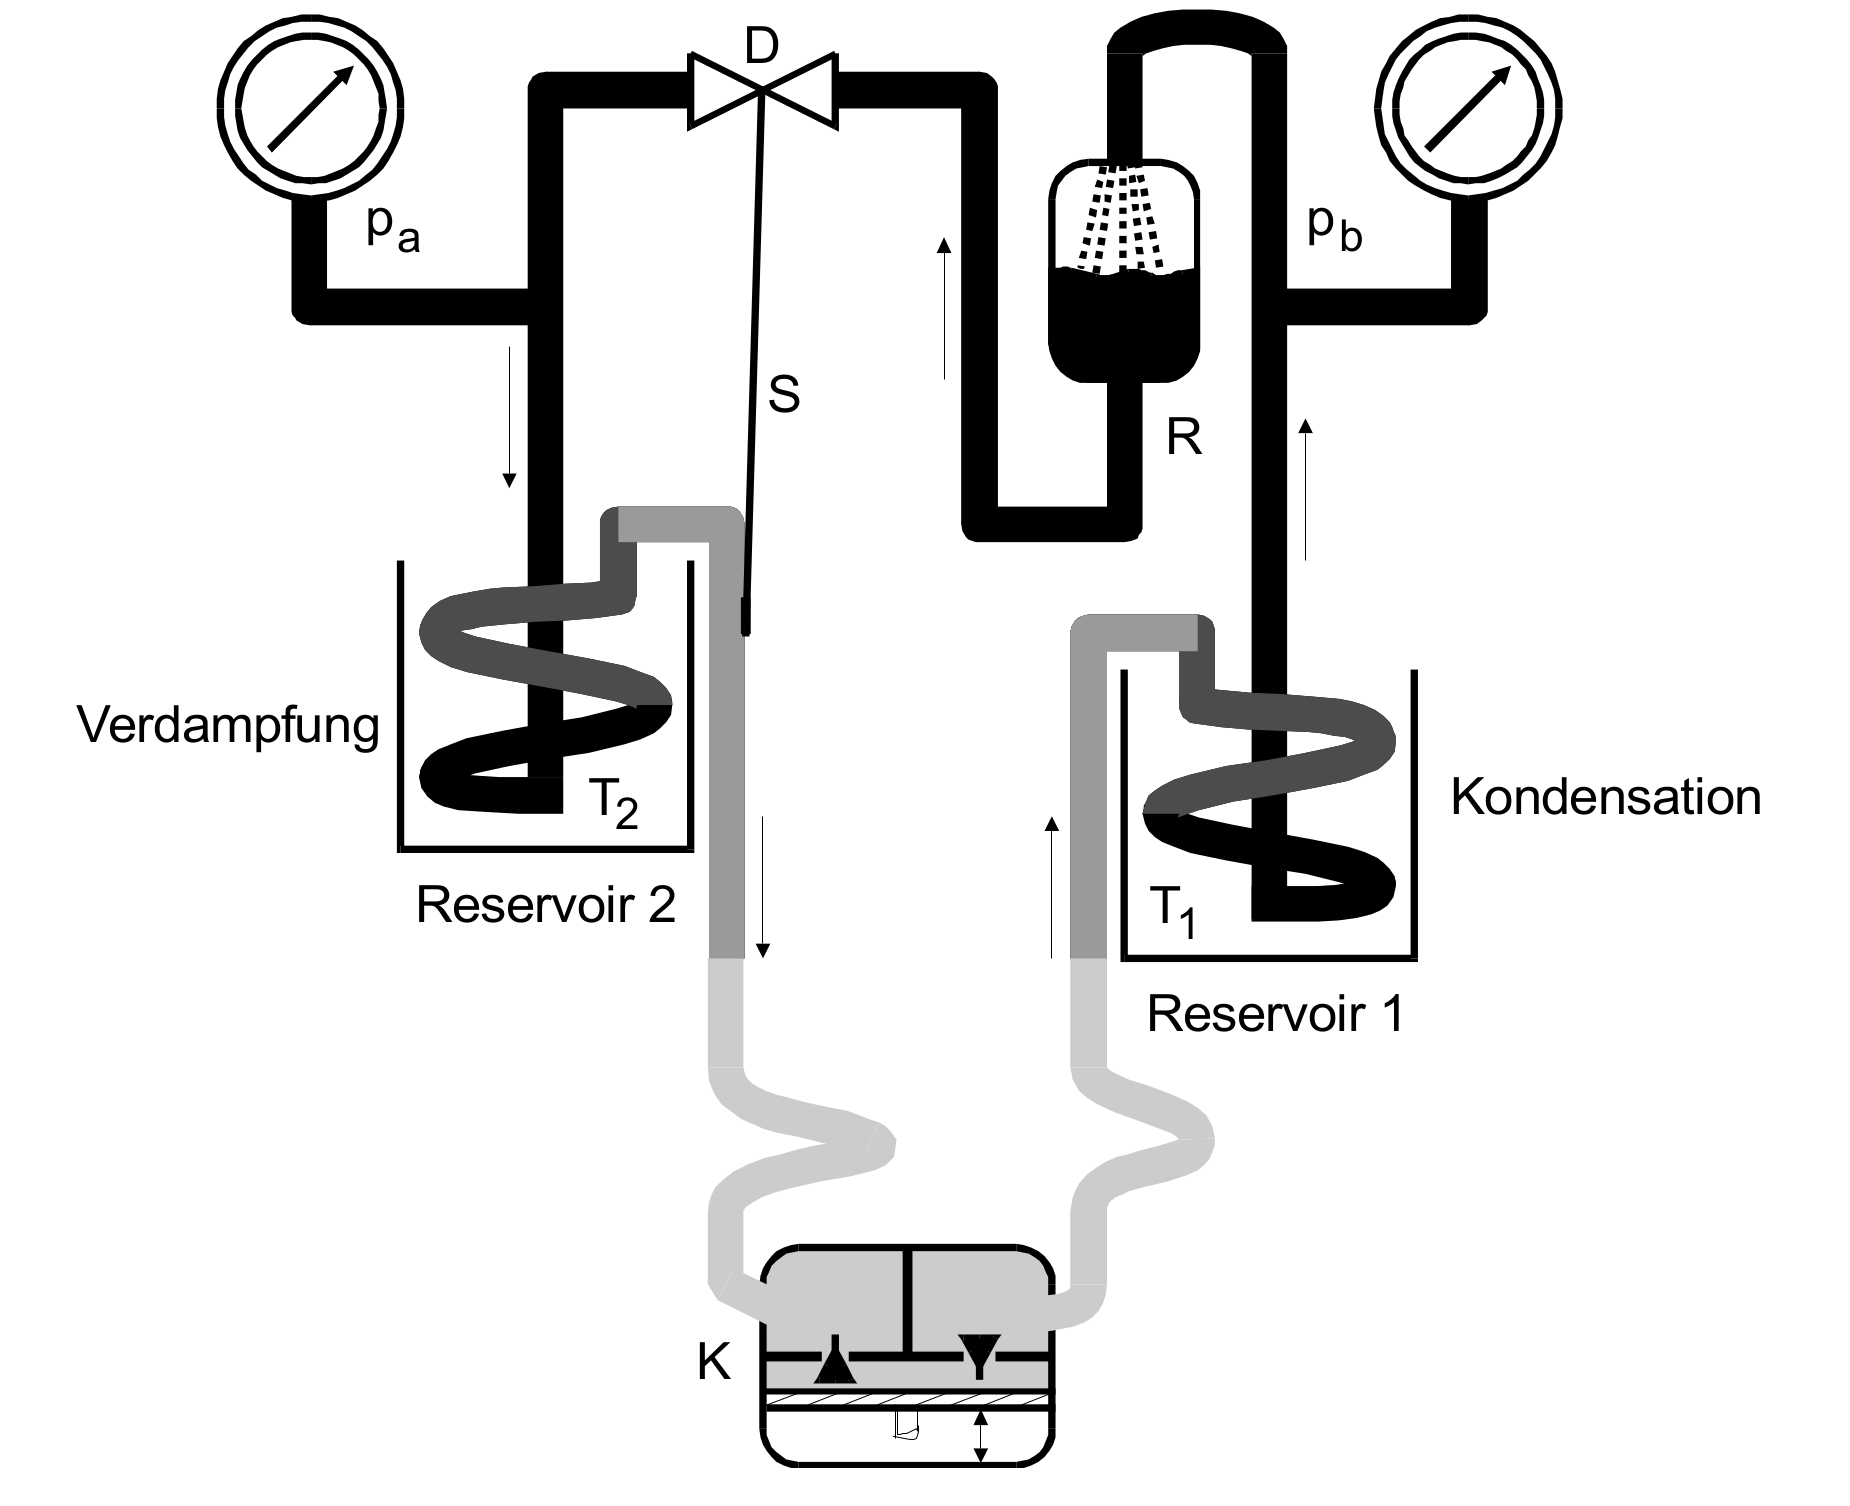
\includegraphics[scale = 0.15]{AufbauWaermepumpe.png}
        \caption{Schematische Darstellung einer Wärmepumpe.}
        \label{fig:wärmepumpe1}
      \end{figure}
      In Abbildung \ref{fig:wärmepumpe1} stellen die schwarz eingefärbten Leitungen den Abschnitt dar, in welchem das Transportmedium flüssig ist.
      Aus Reservoir 1 heraus fließt das Transportmedium mit Druck $p_\text{b}$ hinein in den Reiniger R, wo aus dem Transportmedium alle Gasreste entfernt werden.
      Das gereinigte Medium gelangt durch das Drosselventil D. Durch den Strömungswiderstand des Ventils ändert sich der Druck auf $p_\text{a}$. Da das Medium bei Druck $p_\text{b}$
      flüssig, bei Druck $p_\text{a}$ jedoch gasförmig ist, verdampft das Medium in Reservoir 2 bei Temperatur $T_\text{2}$ und nimmt dabei Wärme auf. Die grau eingefärbten Leitungen
      stellen nun den Abschnitt dar, in dem das Transportmedium gasförmig ist. Der Kompressor K komprimiert das Transportmedium adiabatisch,
      wodurch sowohl Temperatur als auch Druck ansteigen.
      In Reservoir 1 kondensiert das Medium wieder und gibt seine Wärmeenergie ab. Die Temperatur $T_\text{1}$ wird erhöht, das
      Transportmedium ist wieder flüssig. Als Transportmedium wird ein reales Gas verwendet.
    \subsection{Durchführung}
      Die Messapparatur ist wie folgt aufgebaut:
      \begin{figure}
        \centering
        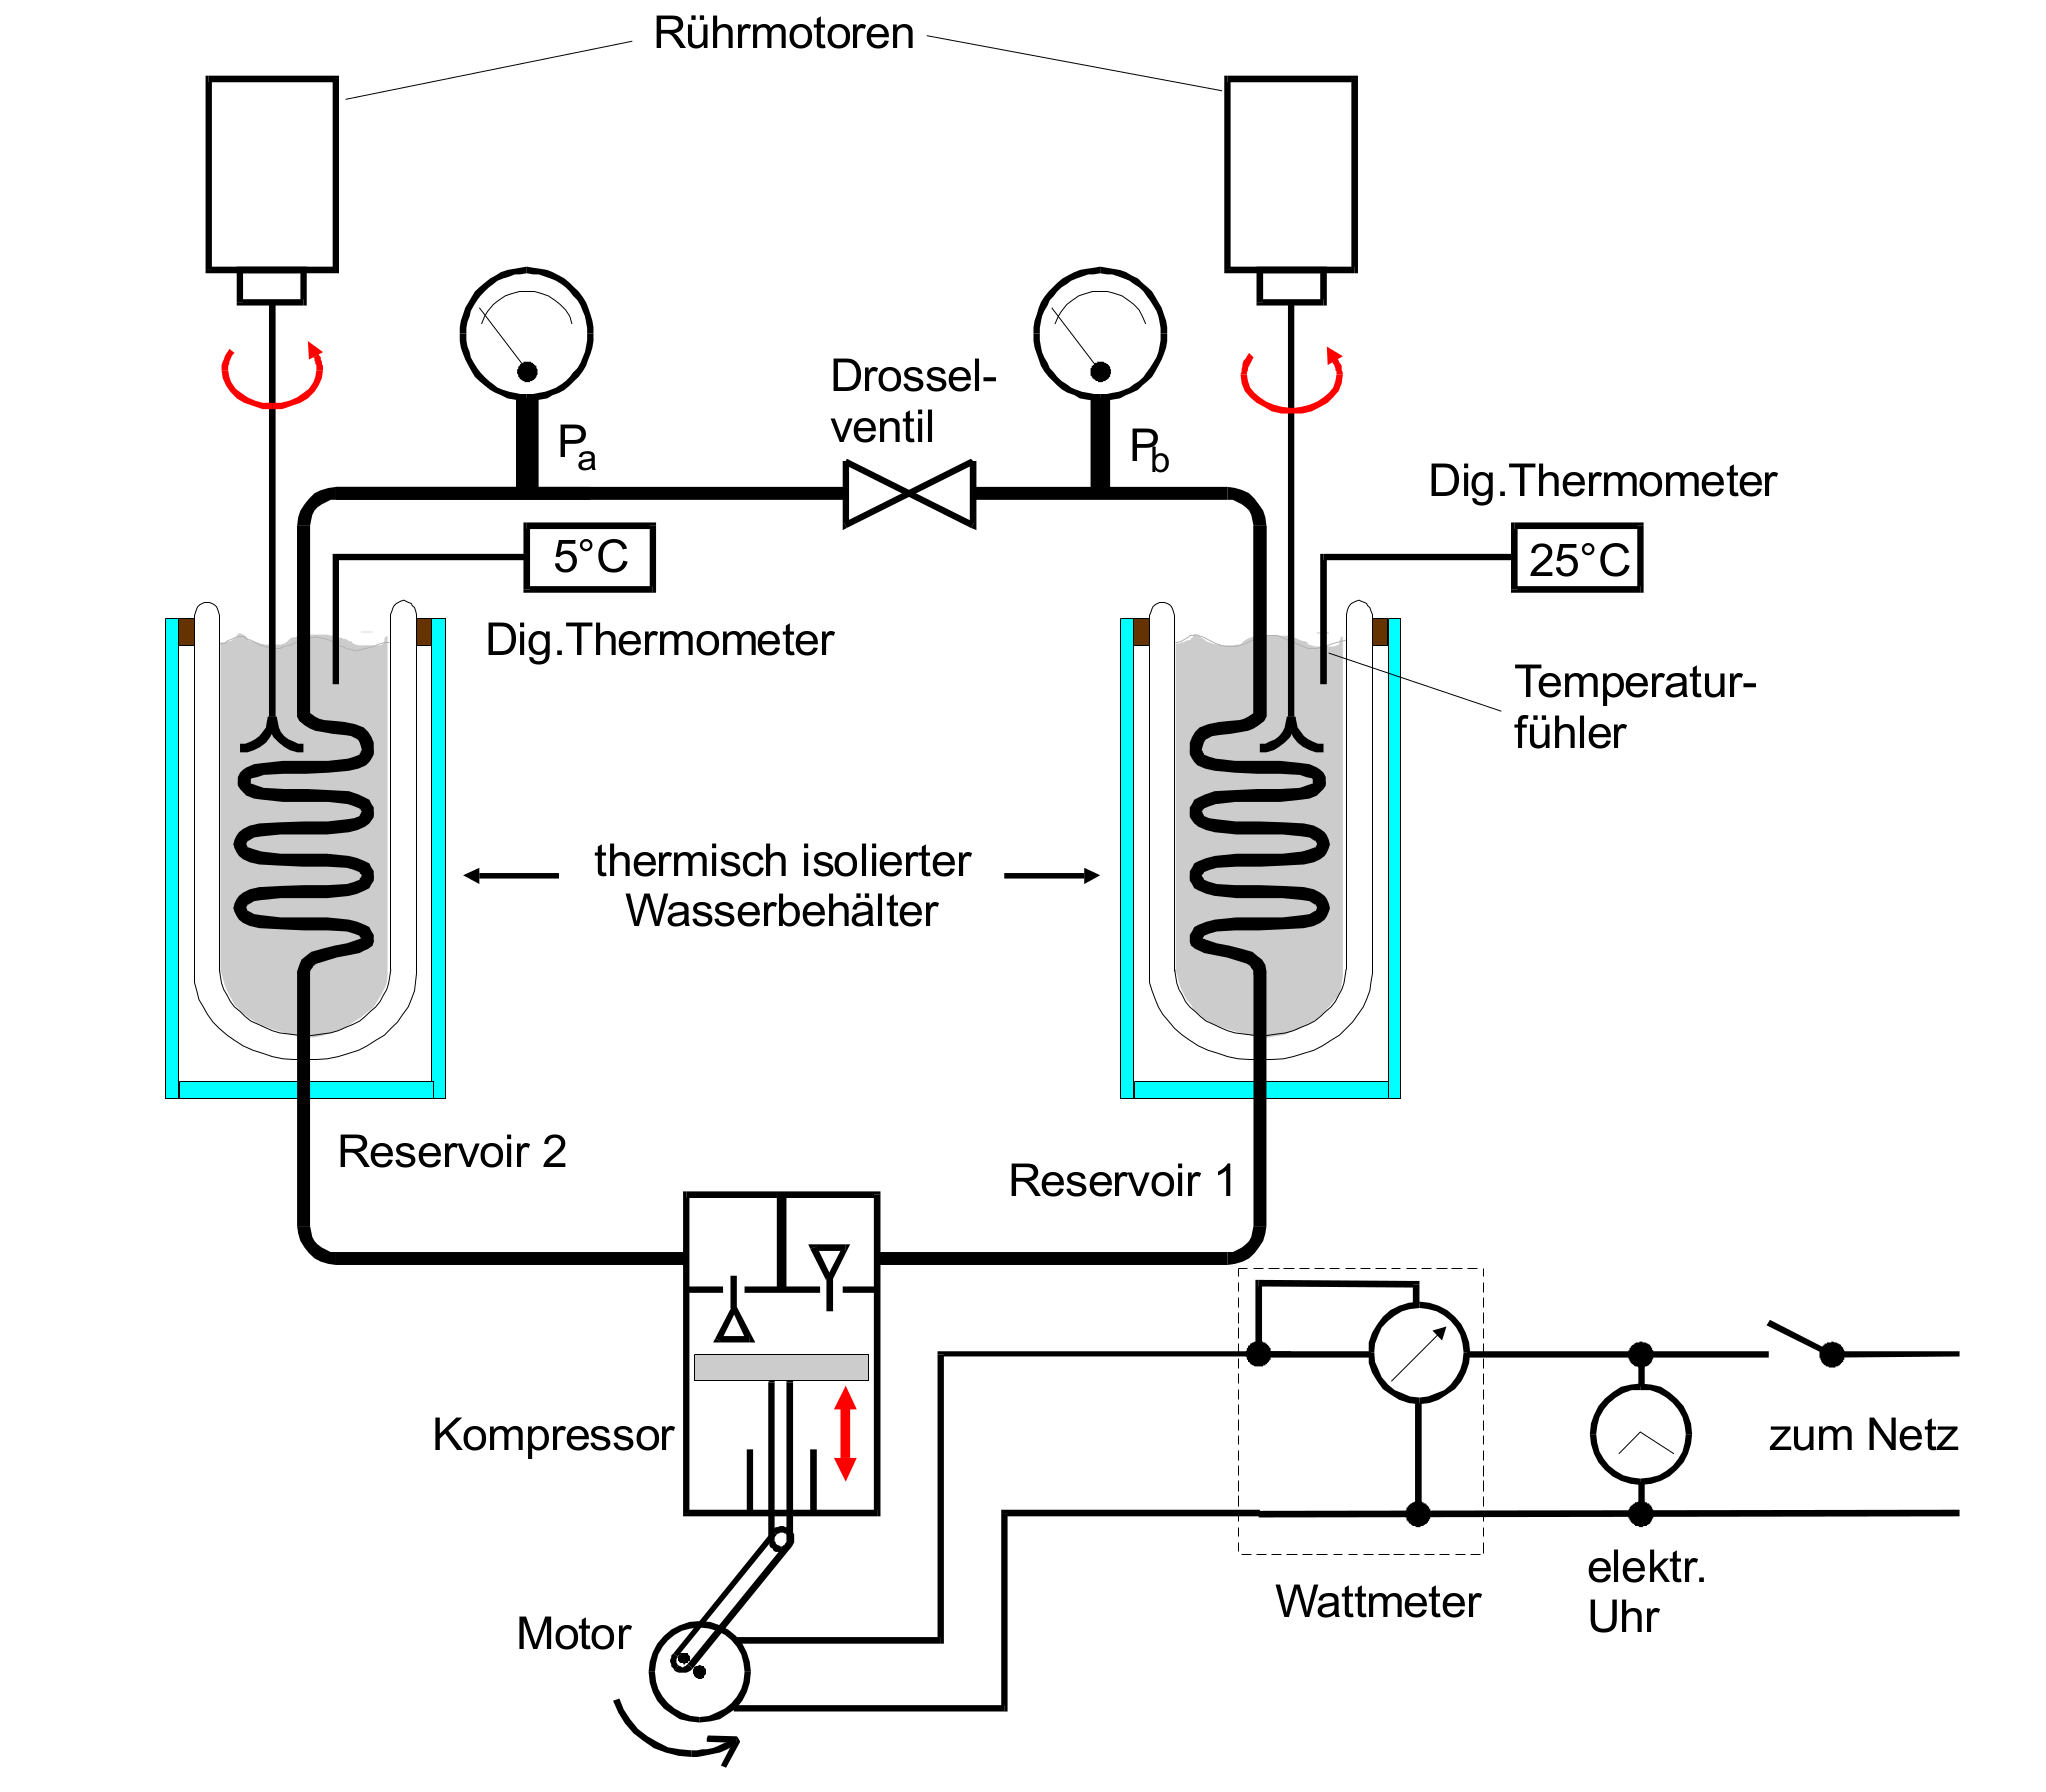
\includegraphics[scale = 0.15]{AufbauMessreihe.png}
        \caption{Die Messapparatur.}
        \label{fig:wärmepumpe2}
      \end{figure}
      In die thermisch isolierten Reservoir 1 und 2 wird eine genau abgemessene Menge kaltes Wasser gefüllt. Damit eine zuverlässige Temperaturmessung mithilfe der beiden
      Digitalthermometer stattfinden kann, werden die Reservoire mit den Rührmotoren während des Experiments laufend durchgerührt. Die Drücke $p_\text{b}$ und $p_\text{a}$
      vor und hinter dem Drosselventil und die Leistungsaufnahme des Kompressors werden ebenfalls aufgenommen. Alle Messwerte werden in Abhängigkeit der Zeit gemessen.
      Jede Minute wurde eine Messung gemacht, bis Reservoir 1 eine Temperatur von $T_\text{1} = \SI{50}{\celsius}$ erreicht hat.
\section{Ergebnisse des Experiments}
    \subsection{Diskussion der Ergebnisse}
    Es fällt auf, das die errechnete Güteziffer der Wärmepumpe relativ weit von der idealen abweicht, siehe \ref{tab:güteziffer}. Dies liegt vermutlich an der Isolierung der
    Reservoire, die einen Wärmeaustausch mit der Umgebung nicht vollständig verhindern kann. Außerdem läuft die Kompression nur annähernd adiabatisch ab, hier treten also weitere
    Verluste auf. Zudem haben wir die Messung nicht selber durchgeführt, möglicherweise ist auch die Genauigkeit der Messung in Zweifel zu ziehen.
\end{document}

%\eqref{eqn:}